%!TEX root = bachelor.tex

\chapter{Mathematica-Modell}%
\label{appendix:mathematica}

Das für die numerische Berechnung in \cref{sec:other:numeric} erstelle Mathematica-Modell ist in \cref{tbl:mathematica} dargestellt. In der ersten Eingabezeile werden zunächst die Randbedingungen für die Parameter $q$, $r_1$, $r_2$, $d$ und $s$ gesetzt. Die Eingabezeilen~2 bis~5 modellieren die \cref{eqn:div:boarder1,eqn:div:boarder2} auf \cpageref{eqn:div:boarder1}. In Zeile~6 wird die zu untersuchende Verteilungsfunktion festgelegt. Das Beispiel nutzt eine Gleichverteilung über dem Intervall $[0,s]$, wie es auch von \Citeauthor{Wagner-2010} betrachtet wird. Die Verteilung lässt sich an der Stelle jedoch durch eine beliebige andere Verteilungsfunktion ersetzen, wie in \cref{sec:other:numeric} geschehen. In den Zeilen~7 \bzw{}~8 werden die Funkionen $\pi_2$ \bzw{} $\pi^S$ modelliert. Hierbei ist anzumerken, dass die Integrale bereits hier soweit wie möglich ausgewertet werden, um diese Rechnung nur einmalig durchführen zu müssen und nicht bei jeder folgenden Bestimmung der optimalen Diversifikationsgrade erneut. Insbesondere für komplexere Verteilungsfunktionen stellt dieser Schritt einer der rechenintensivsten dar.

In den Eingabezeilen~9 und folgenden werden die optimalen Diversifikationsgrade sowohl bezüglich der Volkswirtschaft ($r^\ast$) als auch die individuellen ($r^E$) numerisch bestimmt. Um moderne multi-core Rechner effizient nutzen zu können, finden die Berechnungen für verschiedene Modellparameter parallel statt. Im Beispiel in \cref{tbl:mathematica} wird der Parameter $q$ zwischen 1,1 und 10 variiert. Um die Komplexität der einzelnen Berechnungen besser abschätzen zu können, wird gleichzeitig die Rechenzeit erhoben. Die Ergebnisse der numerischen Optimierung werden schlussendlich in einer Tabelle wie im Beispiel in Ausgabezeile~11 ausgegeben zusammen mit der Gesamtrechenzeit in Zeile~12.

\begin{sidewaystable}[t!]
	\centering
	\caption{Mathematica-Modell zur numerischen Bestimmung der optimalen Diversifikationsgrade.}%
	\label{tbl:mathematica}
	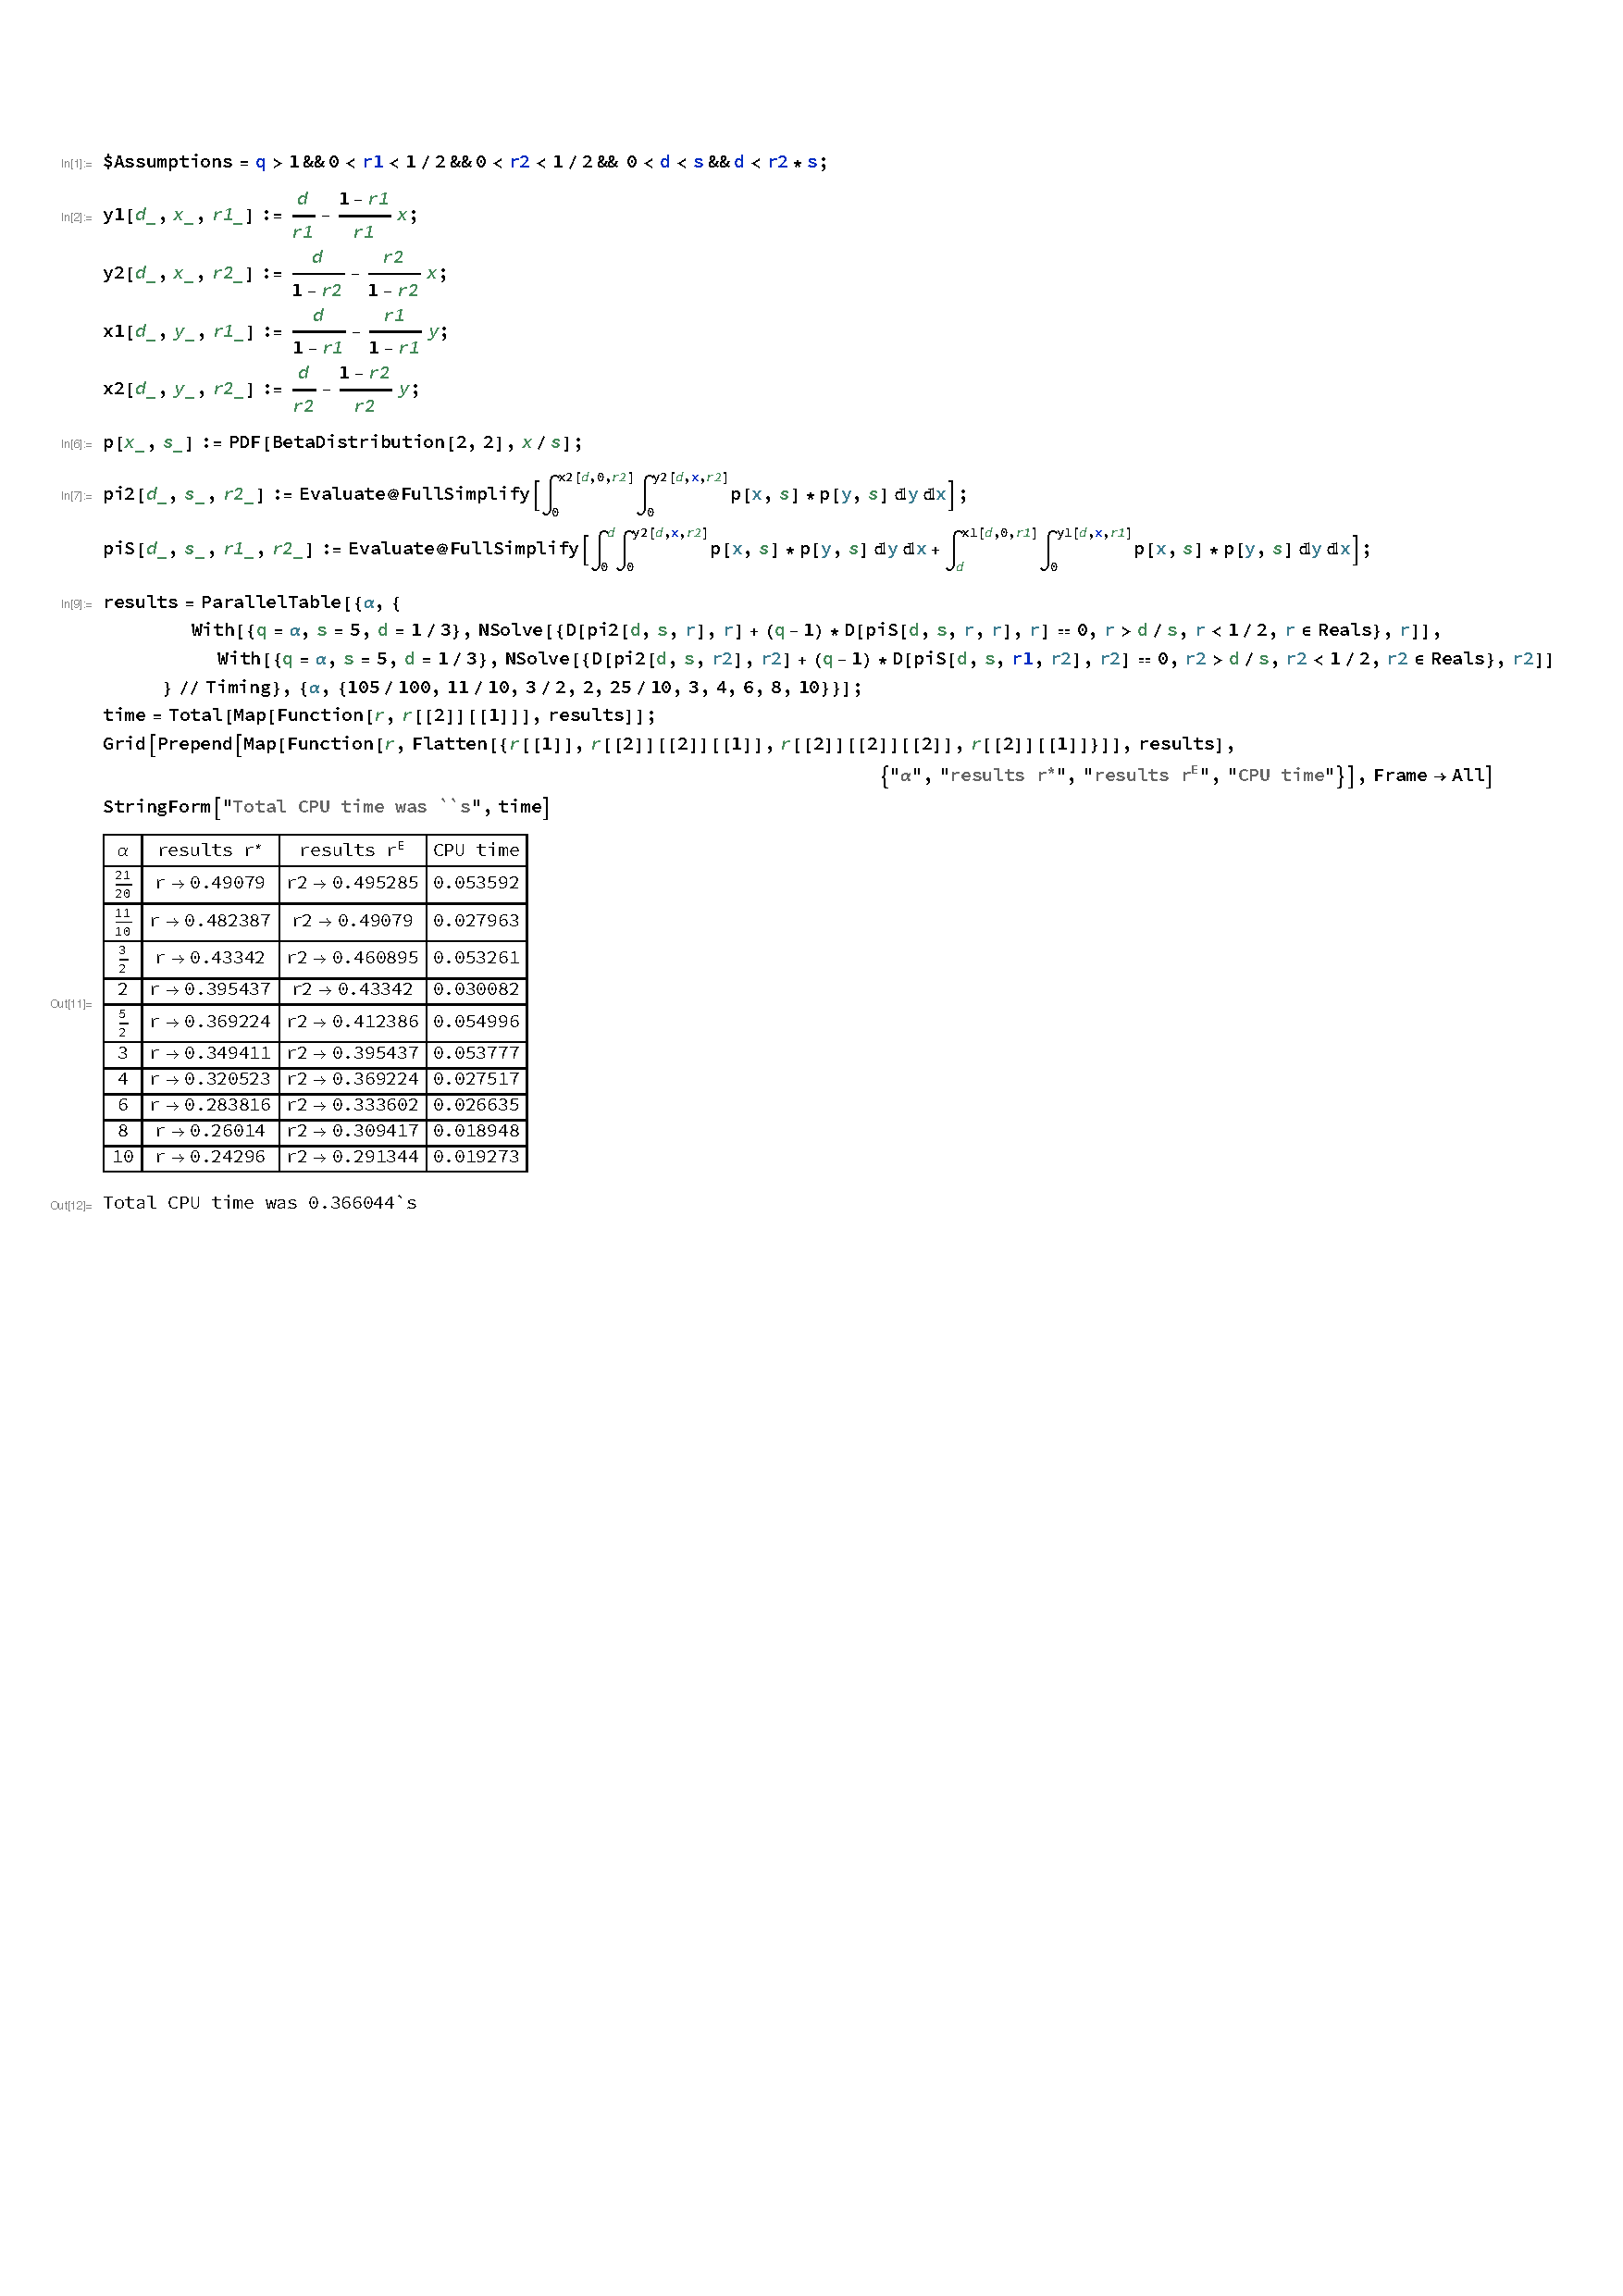
\includegraphics[scale=0.7]{figures/mathematica-source}
\end{sidewaystable}